\documentclass{article}

% Language setting
% Replace `english' with e.g. `spanish' to change the document language
\usepackage[english]{babel}

% Set page size and margins
% Replace `letterpaper' with `a4paper' for UK/EU standard size
\usepackage[letterpaper,top=2cm,bottom=2cm,left=3cm,right=3cm,marginparwidth=1.75cm]{geometry}

% Useful packages
\usepackage{amsmath}
\usepackage{mathtools}
\usepackage{graphicx}
\usepackage[colorlinks=true, allcolors=blue]{hyperref}
\usepackage{algorithm}
\usepackage{algpseudocode}
\usepackage{enumitem}
\usepackage{bbm}
\usepackage{comment}

\usepackage{tikz}
\usepackage{pgfplots}
\usetikzlibrary{positioning} 
\usetikzlibrary{calc}
\usetikzlibrary {arrows.meta,bending}
\usetikzlibrary{intersections} %<-added
\usepgfplotslibrary{fillbetween} %<-added
\pgfplotsset{compat=1.11}

  \tikzset{
    pics/ig_tree/.style args = {#1, #2}{% name, label
      code = {
        \draw[draw=blue!60, dashed, fill=blue!5, very thick] (-0.2, -0.2) rectangle (1.2, 1.2);
        \draw[draw=red!60, fill=red!5, very thick] (0, 0) rectangle node[pos=0.5] (#1) {#2} (1, 1);
      }
    }
  }
  
  \tikzset{ 
    pics/ig_tree_region/.style args = {#1, #2, #3}{% name, label
      code = {
        \draw[draw=#3!100, fill=#3] (#1) rectangle (#2);
      }
    }
  }
  

\newcommand{\oldB}[2]{\prescript{#1}{}{\mathcal{B}}^\textrm{old}_#2}
\newcommand{\newB}[2]{\prescript{#1}{}{\mathcal{B}}^\textrm{new}_#2}

\title{Parthenon Notes}
\author{You}

\begin{document}

\maketitle

Here we collect some notes about the implementation of selected aspects of \texttt{Parthenon}.
\tableofcontents 

\section{Forest of Octrees} 

To allow more complex topological meshes than are currently supported\footnote{The \texttt{Athena++} implementation  of octree AMR limits domains to having a logically hyper-rectangular shape.}, we would like to go to a forest of octrees type approach. We can then think of a topological macromesh of trees that share faces, edges, and nodes. The goal is to support an arbitrarily connected hexahedral macrosmesh, which implies that trees can have one tree neighbor per face, but an arbitrary number of edge and node connections (including zero even on internal elements). Additionally, the logical coordinate systems of the trees do not necessarily align, so it is necessary to encode information about the relative connectivity of the blocks with shared elements. 

A forest of octrees covering a manifold $\mathcal{M}$ is defined by a set of nodes, $\mathcal{N}$, and a set of faces, $\mathcal{F}$ (in 2D) or cells $\mathcal{C}$ (in 3D) that each contain an octree. Each face corresponds to a 4-tuple of nodes, $f_i$ and each cell corresponds to an 8-tuple of nodes, $c_i$. For now, we do not attach any further geometric information to the forest. Rather, we just assume that there exist integer grid maps $g_i: \Omega_i \rightarrow \mathcal{M}_i$, where $\mathcal{M}_i \in \mathcal{M}$ is the region of the manifold covered by face (cell) $i$ and $\Omega_i \in \Omega$ is a square (cubic) region of an integer grid $\Omega$ that is bounded by integer grid lines (planes) separated by one unit. The ghost halos and interiors of the the trees are connected by logical coordinate transformations $\tau_{i \rightarrow j}$.
\begin{center}
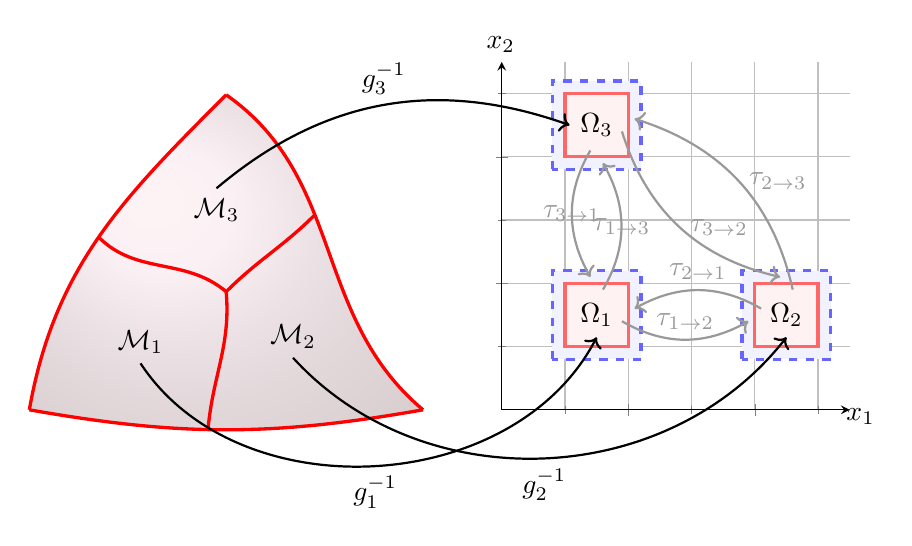
\begin{tikzpicture}[line/.style={red, very thick}]
\coordinate (m2) (10.0, 0.0);

\coordinate (n1) at (0,0); 
\coordinate (n2) at (5,0);
\coordinate (n3) at (2.5,4);
\coordinate (n4) at (2.5,1.5);

\fill[fill=red!5] (n1) to[out=-10,in=190] (n2) to[out=140,in=-35] (n3) to[out=-135,in=80] cycle;
\shade[ball color=blue!10!white,opacity=0.20] (n1) to[out=-10,in=190] (n2) to[out=140,in=-35] (n3) to[out=-135,in=80] cycle;

\draw[line] (n1) to[out=-10,in=190] coordinate[pos=.45] (m12) (n2);
\draw[line] (n2) to[out=140,in=-35] coordinate[pos=.6] (m23) (n3);
\draw[line] (n3) to[out=-135,in=80] coordinate[pos=.5] (m31) (n1);

\draw[line] (n4) to[out=-85,in=85] (m12);
\draw[line] (n4) to[out=45,in=225] (m23);
\draw[line] (n4) to[out=140,in=-45] (m31);

\node (m1) at ($0.25*(n1) + 0.25*(m12) + 0.25*(n4) + 0.25*(m31)$) {$\mathcal{M}_1$};
\node (m2) at ($0.25*(m12) + 0.25*(n2) + 0.25*(m23) + 0.25*(n4)$) {$\mathcal{M}_2$};
\node (m3) at ($0.25*(n4) + 0.25*(m23) + 0.25*(n3) + 0.25*(m31)$) {$\mathcal{M}_3$};

\begin{axis}[grid=both,
             ymin=0,
             ymax=5.5,
             xmax=5.5,
             xmin=0,
             xticklabel=\empty,
             yticklabel=\empty,
             minor tick num=1,
             axis lines = middle,
             xlabel=$x_1$,
             ylabel=$x_2$,
             label style = {at={(ticklabel cs:1.1)}}, 
             axis equal=true, 
             at={(6cm, 0)},
             width=6.0cm, height=6.0cm]

  \coordinate (t1ll) at (1, 1);
  \pic at (t1ll) {ig_tree={t1, $\Omega_1$}};

  \coordinate (t2ll) at (4, 1);
  \pic at (t2ll) {ig_tree={t2, $\Omega_2$}};

  \coordinate (t3ll) at (1, 4);
  \pic at (t3ll) {ig_tree={t3, $\Omega_3$}};

  \path[thick, ->, black!40] ([shift={(0.9,0.4)}]t1ll) edge[bend right] 
          node [above] {$\tau_{1 \rightarrow 2}$} ([shift={(-0.1,0.4)}]t2ll);
  \path[thick, ->, black!40] ([shift={(0.1,0.6)}]t2ll) edge[bend right] 
          node [above] {$\tau_{2 \rightarrow 1}$} ([shift={(1.1,0.6)}]t1ll);

  \path[thick, ->, black!40] ([shift={(0.6,0.9)}]t2ll) edge[bend right] 
          node [right] {$\tau_{2 \rightarrow 3}$} ([shift={(1.1,0.6)}]t3ll);
  \path[thick, ->, black!40] ([shift={(0.9,0.4)}]t3ll) edge[bend right] 
          node [right] {$\tau_{3 \rightarrow 2}$} ([shift={(0.4, 1.1)}]t2ll);
  
  \path[thick, ->, black!40] ([shift={(0.4,0.1)}]t3ll) edge[bend right] 
          node [] {$\tau_{3 \rightarrow 1}$} ([shift={(0.4, 1.1)}]t1ll);
  \path[thick, ->, black!40] ([shift={(0.6,0.9)}]t1ll) edge[bend right] 
          node [] {$\tau_{1 \rightarrow 3}$} ([shift={(0.6, -0.1)}]t3ll);        
\end{axis}

\path[thick, ->] (m1.south) edge[bend right = 60] node [below] {$g_1^{-1}$} (t1.south);
\path[thick, ->] (m2.south) edge[bend right = 50] node [below] {$g_2^{-1}$} (t2.south);
\path[thick, ->] (m3.north) edge[bend left] node [above] {$g_3^{-1}$} (t3.west);
\end{tikzpicture}
\end{center}


By construction, these maps take the nodes of a 4-tuple (8-tuple) defining a face (cell) to the corners of a square (cube) in morton-order. We define logical coordinates to be coordinates defined on this integer grid\footnote{Formally it is probably necessary to define numerous coordinate systems on the integer grid, both associated with each block (which differ by only a translation) and with each octree level in a block (which differ by a scaling factor of $2^\ell$ where $\ell$ is the refinement level of the octree), but we aren't explicit about that here.}. The index of each node in an 8-tuple defining a block are
\begin{center}
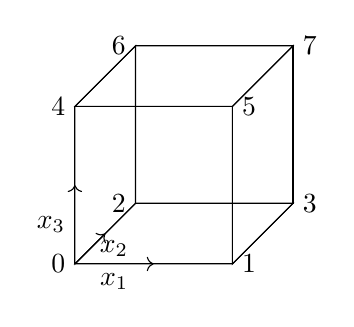
\begin{tikzpicture}
\newcommand{\Depth}{2}
\newcommand{\Height}{2}
\newcommand{\Width}{2}
\coordinate (O) at (0,0,0);
\coordinate (A) at (0,\Width,0);
\coordinate (B) at (0,\Width,\Height);
\coordinate (C) at (0,0,\Height);
\coordinate (D) at (\Depth,0,0);
\coordinate (E) at (\Depth,\Width,0);
\coordinate (F) at (\Depth,\Width,\Height);
\coordinate (G) at (\Depth,0,\Height);

\draw[black] (O) node [left]{2} -- (C) node [left]{0} -- (G) node [right]{1} -- (D) node [right]{3} -- cycle;% Bottom Face
\draw[black] (O) -- (A) -- (E) -- (D) -- cycle;% Back Face
\draw[black] (O) -- (A) -- (B) -- (C) -- cycle;% Left Face
\draw[black] (D) -- (E) -- (F) -- (G) -- cycle;% Right Face
\draw[black] (C) -- (B) -- (F) -- (G) -- cycle;% Front Face
\draw[black] (A) node [left]{6} -- (B) node [left]{4} -- (F) node [right]{5}-- (E) node [right]{7} -- cycle;% Top Face

\path[->] ([shift={(0,0,0)}]C) edge node [below] {$x_1$} ([shift={(-1.0, 0, 0)}]G);
\path[->] ([shift={(0,0,0)}]C) edge node [right] {$x_2$} ([shift={(0, 0, 1.0)}]O);
\path[->] ([shift={(0,0,0)}]C) edge node [left] {$x_3$} ([shift={(0, -1.0, 0)}]B);
%\draw[blue, fill=black] (1.0, 2.0, 1.0) circle (0.05) node[above] {$(0, 0, 1)$};
%\draw[blue, fill=black] (1.0, 0.0, 1.0) circle (0.05) node[below] {$(0, 0, -1)$};
%\draw[blue, fill=black] (2.0, 1.0, 1.0) circle (0.05) node[right] {$(1, 0, 0)$};
%\draw[blue, fill=black] (0.0, 1.0, 1.0) circle (0.05) node[left] {$(-1, 0, 0)$};
\end{tikzpicture}
\end{center}
The node indices of a 4-tuple defining a face are just the indices of the bottom face. We also require offsets relative to the cell center that are defined by 3-tuples of integers, some examples of offsets are
\begin{center}
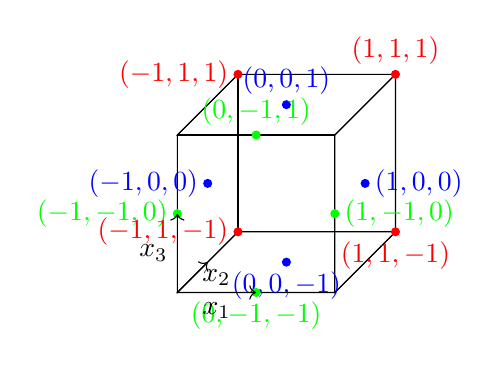
\begin{tikzpicture}
\newcommand{\Depth}{2}
\newcommand{\Height}{2}
\newcommand{\Width}{2}
\coordinate (O) at (0,0,0);
\coordinate (A) at (0,\Width,0);
\coordinate (B) at (0,\Width,\Height);
\coordinate (C) at (0,0,\Height);
\coordinate (D) at (\Depth,0,0);
\coordinate (E) at (\Depth,\Width,0);
\coordinate (F) at (\Depth,\Width,\Height);
\coordinate (G) at (\Depth,0,\Height);

\draw[black] (O) node [left]{} -- (C) node [left]{} -- (G) node [right]{} -- (D) node [right]{} -- cycle;% Bottom Face
\draw[black] (O) -- (A) -- (E) -- (D) -- cycle;% Back Face
\draw[black] (O) -- (A) -- (B) -- (C) -- cycle;% Left Face
\draw[black] (D) -- (E) -- (F) -- (G) -- cycle;% Right Face
\draw[black] (C) -- (B) -- (F) -- (G) -- cycle;% Front Face
\draw[black] (A) node [left]{} -- (B) node [left]{} -- (F) node [right]{}-- (E) node [right]{} -- cycle;% Top Face

\draw[blue, fill=blue] (1.0, 2.0, 1.0) circle (0.05) node[above] {$(0, 0, 1)$};
\draw[blue, fill=blue] (1.0, 0.0, 1.0) circle (0.05) node[below] {$(0, 0, -1)$};
\draw[blue, fill=blue] (2.0, 1.0, 1.0) circle (0.05) node[right] {$(1, 0, 0)$};
\draw[blue, fill=blue] (0.0, 1.0, 1.0) circle (0.05) node[left] {$(-1, 0, 0)$};
%\draw[blue, fill=black] (1.0, 1.0, 2.0) circle (0.05) node[right] {$(0, 1, 0)$};
%\draw[blue, fill=black] (1.0, 1.0, 0.0) circle (0.05) node[left] {$(0, -1, 0)$};

\draw[green, fill=green] (1.0, 2.0, 2.0) circle (0.05) node[above] {$(0, -1, 1)$};
\draw[green, fill=green] (1.0, 0.0, 2.0) circle (0.05) node[below] {$(0, -1, -1)$};
\draw[green, fill=green] (2.0, 1.0, 2.0) circle (0.05) node[right] {$(1, -1, 0)$};
\draw[green, fill=green] (0.0, 1.0, 2.0) circle (0.05) node[left] {$(-1, -1, 0)$};

\draw[red, fill=red] (2.0, 2.0, 0.0) circle (0.05) node[above] {$(1, 1, 1)$};
\draw[red, fill=red] (2.0, 0.0, 0.0) circle (0.05) node[below] {$(1, 1, -1)$};
\draw[red, fill=red] (0.0, 2.0, 0.0) circle (0.05) node[left] {$(-1, 1, 1)$};
\draw[red, fill=red] (0.0, 0.0, 0.0) circle (0.05) node[left] {$(-1, 1, -1)$};

\path[->] ([shift={(0,0,0)}]C) edge node [below] {$x_1$} ([shift={(-1.0, 0, 0)}]G);
\path[->] ([shift={(0,0,0)}]C) edge node [right] {$x_2$} ([shift={(0, 0, 1.0)}]O);
\path[->] ([shift={(0,0,0)}]C) edge node [left] {$x_3$} ([shift={(0, -1.0, 0)}]B);
\end{tikzpicture}
\end{center}
where offsets corresponding to faces are blue, edges are green, and nodes are red.

%In our conception, the faces can be placed arbitrarily on the integer grid, as long as there are at least two grid positions in between each pair of trees. This only matters formally and for creating a mental model, relative positions on the integer grid are never explicitly specified for faces. The coordinate system associated with each face has an origin at the lower left hand corner. 

Each refinement level, $\ell$, of the octree has a coordinate system that runs from 0 to $2^\ell$ from one side of the face to the other in each direction. We refer to positions one unit outside of $[0, 2^\ell]^D$ as the ghost halo of the tree. A \texttt{LogicalLocation} as defined in \texttt{Parthenon} is an integer D-tuple at level $\ell$ defining the position of the lower left hand corner of a unit cube. If this cube is in the interior of the tree, this level and location can be transformed into a Morton number. This gives a nearly perfect hash for \texttt{LogicalLocation}, which we use to allow us to represent trees as hash maps of leaf node \texttt{LogicalLocation}s using \texttt{std::unordered\_map}.

Similarly to blocks in an octree, it is necessary to allow for each octree itself to have a ghost halo. If a block is refined at the boundary of one octree, this can trigger refinement in a neighboring octree as a result of demanding a properly nested grid. The simplest way to deal with this is to transform the logical location of the newly refined block in the logical coordinate system of the origin block to the logical location in the logical coordinate system of the neighbor block. Therefore, it is necessary to find transformation maps $\vec{u}_{j,\ell} = \tau_{i \rightarrow j}(\vec{u}_{i, \ell})$. Here $\vec{u}_{i, \ell}$ is a coordinate vector in the logical coordinate system of block $i$ at level $\ell$. 

\subsection{Forest Neighbor Connectivity}
To build a \texttt{Mesh} based on a general forest, the unstructured macro-grid of octrees in the forest must first be constructed. In 2D, this macro grid consists of a set of \texttt{std::shared\_ptr<forest::Node>}s and a set of \texttt{std::shared\_ptr<forest::Face>}s constructed from 4-tuples of these nodes. This pointer graph is then used to find the neighboring faces and logical coordinate transformations of every face in the forest and associate boundary conditions with edges that are unshared. Then, a \texttt{forest::Forest} object can be built that includes a set of \texttt{forest::Tree}s that store the neighbor connection information. \texttt{Mesh} contains a constructor that takes a \texttt{ForestDefinition} (which just contains a list of faces, boundary conditions, initial refinement locations, and the physical coordinates of each tree) and builds a \texttt{Mesh} based on this general topology. Since the macro-mesh is not adaptive, this procedure occurs only once at the beginning of a simulation (or at the beginning of a restart). 

\subsubsection{Finding Neighbors}
Finding node, edge and face neighbors in the forest is very straightforward. First, associate every face that contains a given node with that node (in practice this is done by giving each node a vector of pointers to faces that contain it). Then for each face (cell) $i$, go through each node in $f_i$ and get the set of associated faces $\{f_j\} / f_i$ (cells $\{c_j\} / c_i$). Take the intersection of $f_i$ with each $f_j$. If there is one node in the intersection, $f_j$ is a corner neighbor, if there are two nodes in the intersection and they correspond to an edge of face $i$ and of face $j$ the two are edge neighbors, etc. There are a number of checks that can be done here for the realizability of the mesh. 

\subsubsection{Finding face neighbor coordinate transforms}
We define a map that takes a node in a face and returns its index in the 4-tuple defining the face
\begin{equation}
\mathcal{I}_{f_i}: f_i \rightarrow \{0, 1, 2, 3\}.  
\end{equation}
Because of our choice of Morton ordering of the corners, it is easy to see by inspection that the direction of an oriented edge $(n_1, n_2) \in \mathcal{N}^2$ is given by 
\begin{equation}
d_i(n_1, n_2) = \textrm{sign}(\mathcal{I}_{f_i}(n_2) -  \mathcal{I}_{f_i}(n_1)) \left[1 + \log_2 \left |\mathcal{I}_{f_i}(n_2) -  \mathcal{I}_{f_i}(n_1)\right|\right].
\end{equation}
If $\textrm{frac}(d(n_1, n_2)) \neq 0$, then this is not an edge of the face (i.e. $n_1$ and $n_2$ are on opposite corners of the face), otherwise the edge is aligned in the $\hat \imath$ direction if $|d| = 1$ or the $\hat \jmath$ direction if $|d| = 2$ (or the $\hat k$ direction if $|d|=3$ in a 3D forest). If $ d > 0$, the edge points in the same direction as the associated unit vector, otherwise it points in the opposite direction. 

Define the offsets of the nodes of a face as is normally done in Parthenon (e.g. the node at position zero in the tuple has offset $(-1, -1, -1)$ from the center of the tree in 3D). Then, the offset of any component of any component of a cell or face defined from an n-tuple can be found from 
\begin{equation}
\vec{O}_{f_i}[(n_0, ..., n_{n-1})] = \frac{1}{n} \sum_{j=0}^{n-1} \textrm{offset}(\mathcal{I}_{f_i}(n_j)).
\end{equation}
$\vec{O} \cdot \vec{O}$ can easily be checked to make sure that chosen set of nodes actually corresponds to a face (so that $\vec{O} \cdot \vec{O} = 1$) or an edge (so that $\vec{O} \cdot \vec{O} = 1 \textrm{ or } 2$ in 2- and 3D).

Using these results, the procedure for finding the coordinate transformation from an origin octree $o$ to a neighbor octree $n$ 
\begin{equation}
\vec{u}_{n, \ell} = 
\tau_{o \rightarrow n}(\vec{u}_{o, \ell}) = R_{o \rightarrow n} 
(\vec{u}_{o, \ell} - 2^\ell \vec{t}),
\end{equation}
where $R_{o \rightarrow n}$ is a 3x3 orthogonal matrix contained in the full octahedral symmetry group (which has 48 members). $R$ is not explicitly built in \texttt{Parthenon}, rather it is implicitly stored in arrays mapping directions in one coordinate system to directions in the other in the class \texttt{forest::LogicalCoordinateTransformation}. The translation vector $\vec{t}$ is defined for coordinate systems at $\ell = 0$.
This transformation map is associated with a shared edge $(n_a, n_b)$ or a shared face $(n_a, n_b, n_c, n_d)$ is 
\begin{enumerate}
\item Re-orient the shared edge by sorting the tuple based on $\mathcal{I}_{f_o}(n_i)$ so that $(n_a, n_b) \rightarrow (n_0, n_1)$ or $(n_a, n_b, n_c, n_d) \rightarrow (n_0, n_1, n_2, n_3)$.
\item Set the tangential part of the coordinate transformation by associating $d_o(n_0, n_1)$ with $d_n(n_0, n_1)$. In 3D, also do this by associating $d_o(n_0, n_2)$ with $d_n(n_0, n_2)$. (note that both $d_o$ are guaranteed to be positive by virtue of the sorting in step one) 
\item Set the normal part of the coordinate transformation by associating the direction of the non-zero component of $\vec{O}_{f_o}[(n_0, ...)]$ with the direction of the non-zero component of $\vec{O}_{f_i}[(n_0, ...)]$ and setting the sign of the direction positive if the offsets have different sign and negative otherwise.
\item Set the translation $\vec{t} = \vec{O}_{f_o}[(n_0, ...)]$. 
\end{enumerate}

\subsubsection{Finding node neighbor coordinate transforms (2D)}
Because node neighbors only share a single node, there is not enough information to determine a coordinate transformation from one face to the other from the shared node alone. Nevertheless, if another face also includes the node and is an edge neighbor to both faces that are corner neighbors, the coordinate transformation between the node neighbors can be found by composition:
\begin{center}
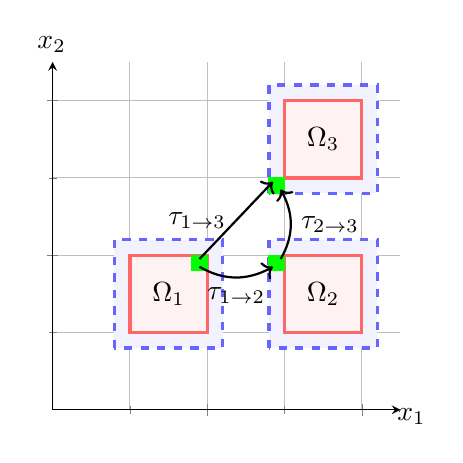
\begin{tikzpicture}
\begin{axis}[grid=both,
             ymin=0,
             ymax=4.5,
             xmax=4.5,
             xmin=0,
             xticklabel=\empty,
             yticklabel=\empty,
             minor tick num=1,
             axis lines = middle,
             xlabel=$x_1$,
             ylabel=$x_2$,
             label style = {at={(ticklabel cs:1.1)}}, 
             axis equal=true, width=6cm, height=6cm]

  \coordinate (t1ll) at (1, 1);
  \pic at (t1ll) {ig_tree={t1, $\Omega_1$}};
  \pic at (t1ll) {ig_tree_region={{0.8, 0.8}, {1.0, 1.0}, green}};

  \coordinate (t2ll) at (3, 1);
  \pic at (t2ll) {ig_tree={t2, $\Omega_2$}};
  \pic at (t2ll) {ig_tree_region={{-0.2, 0.8}, {0.0, 1.0}, green}};

  \coordinate (t3ll) at (3, 3);
  \pic at (t3ll) {ig_tree={t3, $\Omega_3$}};
  \pic at (t3ll) {ig_tree_region={{-0.2, -0.2}, {0.0, 0.0}, green}};

  \path[thick, ->] ([shift={(0.9, 0.85)}]t1ll)  edge[bend right] node [below] 
                   {$\tau_{1 \rightarrow 2}$} ([shift={(-0.15, 0.85)}]t2ll);
  
  \path[thick, ->] ([shift={(-0.05, 0.95)}]t2ll)  edge[bend right] node [right] 
                   {$\tau_{2 \rightarrow 3}$} ([shift={(-0.05, -0.15)}]t3ll);
  
  \path[thick, ->] ([shift={(0.9, 0.95)}]t1ll)  edge node [left] 
                   {$\tau_{1 \rightarrow 3}$} ([shift={(-0.15, -0.05)}]t3ll);
\end{axis}
\end{tikzpicture}
\end{center}
The composition of the coordinate transforms from the origin block $o$ to the share edge neighbor $n'$ followed by the transformation from $n'$ to the corner neighbor $n$ is given by
\begin{equation}
\tau_{o \rightarrow n}(\vec{u}_{o, \ell}) = 
\tau_{n' \rightarrow n}(\tau_{o \rightarrow n'}(\vec{u}_{o, \ell})) = 
R_{n' \rightarrow n} R_{o \rightarrow n'} 
[\vec{u}_{o, \ell} - 2^\ell (\vec{t}_{o \rightarrow n'} + R_{o \rightarrow n'}^{-1}\vec{t}_{n' \rightarrow n})].
\end{equation}
so that 
\begin{equation}
R_{o \rightarrow n} = R_{n' \rightarrow n} R_{o \rightarrow n'} 
\end{equation}
\begin{equation}
t_{o \rightarrow n} = \vec{t}_{o \rightarrow n'} 
+ R_{o \rightarrow n'}^{-1}\vec{t}_{n' \rightarrow n}.
\end{equation}

Therefore, it becomes a straightforward task to build node neighbor coordinate transforms. After sweeping through all faces and calculating and storing edge neighbor transformations, a second sweep through all faces is performed looking for node neighbors. Other faces associated with the shared node are then checked to see if both of the node neighbors are their edge neighbors. Then compositions of the two related coordinate transformations are performed using the routine \texttt{forest::ComposeTransformations}. Note that if we allow for more than five-valent nodes, some transformations require more than a single composition (but the translation should be neglected after the first transformation). 

\subsubsection{Boundary communication in general forests}

When transfering ghost data between blocks that are on separate trees, the buffer can be packed in a different order of positions than the receiving block expects due to the logical coordinate transformation between the trees. To fix this issue, when a receiving block calculates the index space into which it is receiving data it calculates the index space in it own coordinate system then transforms this index range back into the coordinate system of the neighbor block (this transformation only uses the coordinate rotation $R_{o \rightarrow n}^{-1}$ since the translation is already taken care of in the indexing routines). Then, the flattened version of this transformed index space corresponds correctly to the one-dimensional index space of the packed buffer. When the buffer is unpacked, the position of each point in the buffer is transformed back to a position in the logical coordinates of the receiving block using $R_{o \rightarrow n}$. In this way, boundary data is communicated into the correct positions. 

Additionally, the logical coordinate transformations should act on the components of tensorial objects, like some face and edge fields as well as objects with \texttt{Metadata::Vector} and \texttt{Metadata::Tensor}. The code for doing these transformations exists and face- and edge- variables are properly transformed, but transformations are not yet performed on \texttt{Metadata::Vector/Tensor} variables. Currently, all edge and face variables are assumed to be oriented so that their values can change signs in addition to having their indices permuted under some coordinate transformations. This is appropriate if the fields represent represent the normal/tangent components of vectors, but if they just represent a scalar defined on those topological elements there should not be sign changes under the transformation. We need to add a flag that indicates if a field is oriented. 

Five-valent points pose a problem, since two neighbor blocks will want to write data to the corner of a block at a five-valent corner. This has not been dealt with yet in the code, so we are really limited to three- and four-valent corners for now. In the future, the extra data will be stored in a extra index of the variable and be made accessible to downstream codes. For finite-volume codes that reconstruct along coordinate directions, the corner data should never need to be directly accessed but prolongation needs to use it internally at least.

\subsection{Singular valence points}
For a 2D mesh (or an extruded 3D mesh), the allowed topological edge connectivities of each node are 
\begin{center}
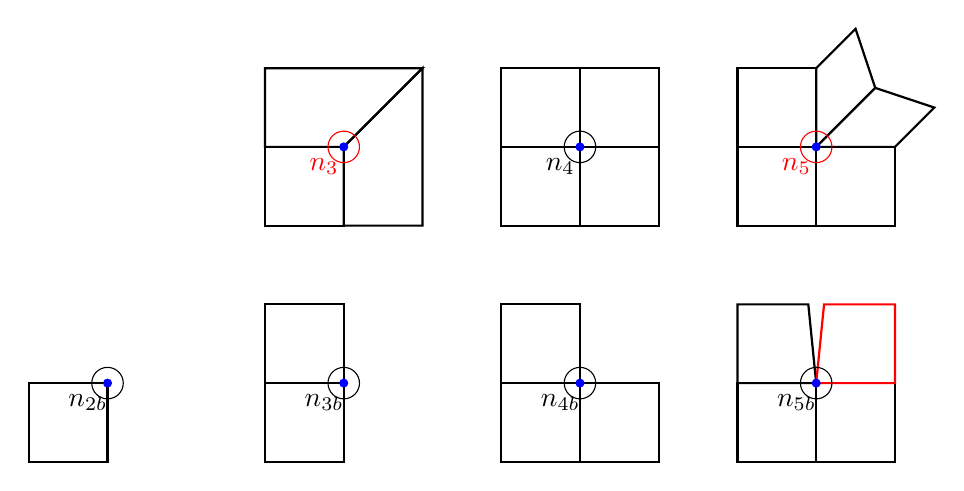
\begin{tikzpicture}
\coordinate (v3) at (3, 0); 
\draw[thick] (v3) -- ([shift={(0, 1)}]v3) -- ([shift={(1, 1)}]v3) -- ([shift={(1, 0)}]v3) -- cycle;
\draw[thick] ([shift={(0, 1)}]v3) -- ([shift={(1, 1)}]v3) -- ([shift={(2, 2)}]v3) -- ([shift={(0, 2)}]v3) -- cycle;
\draw[thick] ([shift={(1, 0)}]v3) -- ([shift={(2, 0)}]v3) -- ([shift={(2, 2)}]v3) -- ([shift={(1, 1)}]v3) -- cycle;
\draw[blue, fill=blue] ([shift={(1, 1)}]v3) circle (0.05);
\draw[red] ([shift={(1, 1)}]v3) circle (0.2) node[shift={(-0.25, -0.25)}] {$n_3$};

\coordinate (v4) at (6, 0); 
\draw[thick] (v4) -- ([shift={(0, 1)}]v4) -- ([shift={(1, 1)}]v4) -- ([shift={(1, 0)}]v4) -- cycle;
\draw[thick] ([shift={(0, 1)}]v4) -- ([shift={(1, 1)}]v4) -- ([shift={(1, 2)}]v4) -- ([shift={(0, 2)}]v4) -- cycle;
\draw[thick] ([shift={(1, 0)}]v4) -- ([shift={(2, 0)}]v4) -- ([shift={(2, 1)}]v4) -- ([shift={(1, 1)}]v4) -- cycle;
\draw[thick] ([shift={(1, 1)}]v4) -- ([shift={(2, 1)}]v4) -- ([shift={(2, 2)}]v4) -- ([shift={(1, 2)}]v4) -- cycle;
\draw[blue, fill=blue] ([shift={(1, 1)}]v4) circle (0.05);
\draw[black] ([shift={(1, 1)}]v4) circle (0.2) node[shift={(-0.25, -0.25)}] {$n_4$};

\coordinate (v5) at (9, 0); 
\draw[thick] (v5) -- ([shift={(0, 1)}]v5) -- ([shift={(1, 1)}]v5) -- ([shift={(1, 0)}]v5) -- cycle;
\draw[thick] ([shift={(0, 1)}]v5) -- ([shift={(1, 1)}]v5) -- ([shift={(1, 2)}]v5) -- ([shift={(0, 2)}]v5) -- cycle;
\draw[thick] ([shift={(1, 0)}]v5) -- ([shift={(2, 0)}]v5) -- ([shift={(2, 1)}]v5) -- ([shift={(1, 1)}]v5) -- cycle;
\draw[thick] ([shift={(1, 1)}]v5) -- ([shift={(2, 1)}]v5) -- ([shift={(2.5, 1.5)}]v5) -- ([shift={(1.75, 1.75)}]v5) -- cycle;
\draw[thick] ([shift={(1, 1)}]v5) -- ([shift={(1, 2)}]v5) -- ([shift={(1.5, 2.5)}]v5) -- ([shift={(1.75, 1.75)}]v5) -- cycle;
\draw[blue, fill=blue] ([shift={(1, 1)}]v5) circle (0.05);
\draw[red] ([shift={(1, 1)}]v5) circle (0.2) node[shift={(-0.25, -0.25)}] {$n_5$};

\coordinate (v1edge) at (0, -3); 
\draw[thick] (v1edge) -- ([shift={(0, 1)}]v1edge) [red]-- ([shift={(1, 1)}]v1edge) [red]-- ([shift={(1, 0)}]v1edge) [black]-- cycle;
\draw[blue, fill=blue] ([shift={(1, 1)}]v1edge) circle (0.05);
\draw[black] ([shift={(1, 1)}]v1edge) circle (0.2) node[shift={(-0.25, -0.25)}] {$n_{2b}$};

\coordinate (v2edge) at (3, -3); 
\draw[thick] (v2edge) -- ([shift={(0, 1)}]v2edge) [red]-- ([shift={(1, 1)}]v2edge) [black]-- ([shift={(1, 0)}]v2edge) -- cycle;
\draw[thick] ([shift={(0, 1)}]v2edge) -- ([shift={(1, 1)}]v2edge) [red]-- ([shift={(1, 2)}]v2edge) [black]-- ([shift={(0, 2)}]v2edge) -- cycle;
\draw[blue, fill=blue] ([shift={(1, 1)}]v2edge) circle (0.05);
\draw[black] ([shift={(1, 1)}]v2edge) circle (0.2) node[shift={(-0.25, -0.25)}] {$n_{3b}$};

\coordinate (v3edge) at (6, -3); 
\draw[thick] (v3edge) -- ([shift={(0, 1)}]v3edge) [red]-- ([shift={(1, 1)}]v3edge) [black]-- ([shift={(1, 0)}]v3edge) -- cycle;
\draw[thick] ([shift={(0, 1)}]v3edge) -- ([shift={(1, 1)}]v3edge) [red]-- ([shift={(1, 2)}]v3edge) [black]-- ([shift={(0, 2)}]v3edge) -- cycle;
\draw[thick] ([shift={(1, 0)}]v3edge) -- ([shift={(2, 0)}]v3edge) -- ([shift={(2, 1)}]v3edge) [red]-- ([shift={(1, 1)}]v3edge) [black]-- cycle;
\draw[blue, fill=blue] ([shift={(1, 1)}]v3edge) circle (0.05);
\draw[black] ([shift={(1, 1)}]v3edge) circle (0.2) node[shift={(-0.25, -0.25)}] {$n_{4b}$};

\coordinate (v4edge) at (9, -3); 
\draw[thick] (v4edge) -- ([shift={(0, 1)}]v4edge) -- ([shift={(1, 1)}]v4edge) -- ([shift={(1, 0)}]v4edge) -- cycle;
\draw[thick] ([shift={(0, 1)}]v4edge) -- ([shift={(1, 1)}]v4edge) [red]-- ([shift={(0.9, 2)}]v4edge) [black]-- ([shift={(0, 2)}]v4edge) -- cycle;
\draw[thick] ([shift={(1, 0)}]v4edge) -- ([shift={(2, 0)}]v4edge) -- ([shift={(2, 1)}]v4edge) -- ([shift={(1, 1)}]v4edge) -- cycle;
\draw[thick] ([shift={(1, 1)}]v4edge) -- ([shift={(2, 1)}]v4edge) -- ([shift={(2, 2)}]v4edge) -- ([shift={(1.1, 2)}]v4edge) [red]-- cycle;
\draw[blue, fill=blue] ([shift={(1, 1)}]v4edge) circle (0.05);
\draw[black] ([shift={(1, 1)}]v4edge) circle (0.2) node[shift={(-0.25, -0.25)}] {$n_{5b}$};
\end{tikzpicture}.
\end{center}
It can be seen that a node can have either zero or two boundary edges that connect to it. Boundary communication across elements of blocks containing nodes of types $n_4$, $n_{2b}$, and $n_{3b}$ is what is currently implemented in Parthenon. Nodes of type $n_{4b}$ are non-singular, but the upper right corner boundary is not filled with using a physical boundary condition in the current infrastructure. Nodes of type $n_{5b}$ also should more or less work with the current infrastructure, although corner data of all blocks at $n_{5b}$ will be ambiguous 

Internal nodes of type $n_3$ and $n_5$ are trickier to deal with. From a purely data communication perspective, points of type $n_3$ should just work, although all blocks will receive no data in the ghost corner corresponding to the $n_3$ node. Nevertheless, if the post communication data is used to prolongate naively using the current implementation the gradients will be calculated using invalid data in the corner, resulting in trash in the ghosts near the $n_3$ point. For nodes of type $n_5$, even data communication does not work since two blocks will be sending data to the corner which would result in a race condition for what data is set there and would once again result in junk for prolongation.  

Some thoughts about 3D meshes:
\begin{itemize}
    \item For 3D, recognizing that a mesh defines a triangulation of an infinitesimal sphere surrounding any given internal node and using Euler's polyhedron formula, we find that the number of cells, $C$, adjacent to the node and the number of edges, $E$, emanating from the node are related by $C = 2(E-2)$ (see \cite{Liu:2018}). If we only allow 3, 4, and 5 valent internal edges, \cite{Liu:2018} shows that the maximum number of edges emanating from a node is 12 so that up to 20 cells can be associated with a node. This is too many, since a single cell associated with the node can only have three face neighbors and six edge neighbors that are all also associated with the node, leaving at least ten neighbor cells that are neighbors via the single vertex of the cell associated with the node. If we limit ourselves to seven or fewer edges emanating from a node, then there are at most three corner neighbors of any possible cell (there are in fact only five different possible topological configurations around a given node \cite{Liu:2018}). 

    \item Another way to think about the allowable configurations is that every neighboring cell of a given cell must be accessible by stepping through at most three faces (similarly to how in 2D we demand that each neighbor face is accessible by stepping through at most two edges). This should limit the valence of the point. How does this look on the triangulation of the sphere mentioned in the previous point? Projected onto the sphere: each edge becomes a node, and each face becomes and edge, and each cell becomes a triangle. So we need to somehow figure out how to throw out triangulations that have more than three step minimal paths between any two triangles. Another way to think about this is how many ways can we triangulate the sphere where we limit ourselves to three, four, and five valent points on the sphere with the additional maximal path constraint. 
    \item Possibly useful: \href{https://www.ams.org/journals/mcom/1967-21-098/S0025-5718-1967-0223277-3/S0025-5718-1967-0223277-3.pdf}{Bowen \& Fisk 1967} show a method for generating triangulations of the sphere from lower node count triangulations of the sphere. Probably can further constrain their algorithm and find the allowed node complexes. Boils down to $\sum_{v \in \{3, 4, 5, ...\}} N_v (6 - v) = 12$ where $N_v$ is the number of nodes with valence $v$ in the triangulation. We would like to limit Some 3-tuples that satisfy this equation are not triangulations, so we need to generate the allowed triangulations with v
\end{itemize}

\section{Geometric Multigrid}
\begin{algorithm}
\caption{Standard multigrid, which results in a matrix form 
\begin{equation*}
M_h = 
\begin{cases}
\tilde S_{h,\text{post}} S_{h,\text{pre}} + S_{h, \text{post}} P_{2h} M_{2h} R_h(I - A_h S_{h, \text{pre}}),& \text{if } h < h_\text{max} \\
A_h^{-1},& \text{if } h \geq h_\text{max},
\end{cases}
\end{equation*}
where $S_{h,\text{pre/post}}$ are smoothers, $R_h$ is a restriction operator from a grid with cell-size $h$ to a grid with cell-size $2h$, $P_{2h}$ is a prolongation operator from $2h$ to $h$, and we have assumed we have a direct solver for our matrix $A$ at the coarsest level.
\label{alg:MG}}
\begin{algorithmic}

\Procedure{MultiGrid$_h$}{$\vec{f}_h$}
    
    \If{$h < h_\text{max}$}
        \State $\vec{u}_h \gets S_{h,\text{pre}} f_h$ \Comment{Requires communication of ghosts before each smoother iteration}
        \State Communicate $\vec{u}_h$ ghosts
        \State $\vec{r}_h \gets f_h - A_h \vec{u}_h$
        \State $\vec{r}_{2h} \gets R_h \vec{r}_h$ \Comment{Restriction doesn't reach across block boundaries}
        \State $\vec{e}_{2h} \gets $ MultiGrid$_{2h}(\vec{r}_{2h})$
        \State Communicate $\vec{e}_{2h}$ ghosts 
        \State $\vec{e}_h \gets P_{2h} \vec{e}_{2h}$ \Comment{Prolongation does reach across block boundaries}
        \State $\vec{u}_h \gets \vec{u}_h + \vec{e}_h$
        \State $\vec{u}_h \gets S_{h,\text{post}} \vec{u}_h$ \Comment{Requires communication of ghosts before each smoother iteration}
    \Else 
        \State $\vec{u}_h \gets A_h^{-1} \vec{f}_{h}$ \Comment{Direct solve on the lowest level}  
    \EndIf
    
    \State \Return $\vec{u}_h$
\EndProcedure 
\end{algorithmic} 
\end{algorithm}

I think this is the original paper about MGCG \cite{Tatebe:1993}. 
The basic multigrid (MG) V-cycle is defined by algorithm~\ref{alg:MG}. As is shown in the comment, MG represents a linear operator on the finest grid that takes the initial RHS $\vec{f}$ and 
returns an approximate solution on the finest level $\vec{u}$. All of the multigrid operators $M_h$ are linear operators that approximately satisfy $M_h \approx A_h^{-1}$ (at least for good choices of $\tilde A_h$ or $S_h$). Then, we can clearly use a multigrid operator as a preconditioner 
\begin{equation}
    A_h \vec{x} = A_h M_h M_h^{-1} \vec{x} = (A_h M_h) \vec{y} = \vec{b} 
\end{equation}
with $\vec{x} = M_h \vec{y}$ or 
\begin{equation}
   (M_h A_h) \vec{x} = M_h \vec{b}. 
\end{equation}

%To test this stuff, we need: 
%\begin{enumerate} 
%\item Block structured mesh with mechanism for ghost communication, simple definition of grid variables and interconnections (all just one dimensional) 
%\item Prolongation and restriction operators 
%\item Actual solution 
%\item Conjugate gradient solver 
%\item Jacobi iteration 
%\item Matrix vector multiplication routines
%\item Simple problem to solve
%\end{enumerate} 

\subsection{Smoothing Operators}
The smoothing operators $S$ generally correspond to a number of iterations of some iterative solver. Here I write down some well known basics, just so I don't forget them. If we are trying to solve the matrix equation $A \vec{x} = \vec{f}$, we can split up the matrix as 
\begin{equation}
    A = P - D 
\end{equation}
so that 
\begin{equation}
\vec{x} = \underbrace{P^{-1} \vec{f}}_{\vec{g}} + \underbrace{P^{-1}D}_R  \vec{x} 
\end{equation} 
If we have an estimate $\vec{x}^{(i)}$ for the true solution $\vec{x}$, we can form a new estimate 
\begin{eqnarray}
    \vec{x}^{(i+1)} &=& \vec{g} + R \vec{x}^{(i)} \nonumber\\
    &=& P^{-1} \left(\vec{f} + D \vec{x}^{(i)} \right),
\end{eqnarray}
this is clearly stationary in the sense that if $\vec{x}^{(i)} = \vec{x}$, then $\vec{x}^{(i+1)} = \vec{x}^{(i)}$.
We can define the error of the estimate as $\vec{\varepsilon}^{(i)} = \vec{x} - \vec{x}^{(i)}$, which gives
\begin{equation}
\vec{\varepsilon}^{(i+m)} = R^m \vec{\varepsilon}^{(i)} 
\end{equation} 
Clearly, for iterations of $R$ to converge to the stationary solution we must have 
\begin{equation}
    \lim_{m \rightarrow \infty} R^m \vec{\varepsilon}^{(0)} = \vec{0} = \sum_i \alpha_i \lambda^m_k \vec{\mathbbm{e}}_k
\end{equation}
which can be stated as 
\begin{equation} 
\rho(R) = \max |\lambda_k| < 1,
\end{equation} 
where $\rho(R)$ is the spectral radius of $R$ (here $\lambda_k$ are the eigenvalues of $R$, $\vec{\mathbbm{e}}_k$ are the corresponding eigenvectors, and $\alpha_i$ are the expansion coefficients of $\vec{\varepsilon}^{0}$ in terms of $\vec{\mathbbm{e}}_k$). So for our relaxation method to theoretically work we require that our split is stationary and has spectral radius less than one. The first part occurs by construction, but the second part doesn't generically hold. 

Assuming $\vec{x}^{(0)} = \vec{0}$, we can write 
\begin{equation}
\vec{x}^{(m)} = \sum_{n=0}^m R^n \vec{g} = \underbrace{\left(\sum_{n=0}^m R^n \right) P^{-1}}_{S} \vec{f} 
\end{equation} 
which makes it clear that this iterative procedure behaves as a linear operator. 

Assume there is an exact solver for each block on on our grid that assumes any pieces of $A$ that reach into ghost zones are zero. Then $P$ could be taken as the combined block local matrices and $D$ would contain the leftover terms of the matrix that couple the blocks through ghosts. Obviously on the root block $D_\text{root} = 0$ and we have an exact solver, so the MG hierarchy can terminate there. 

\begin{figure}[tb]
    \centering
    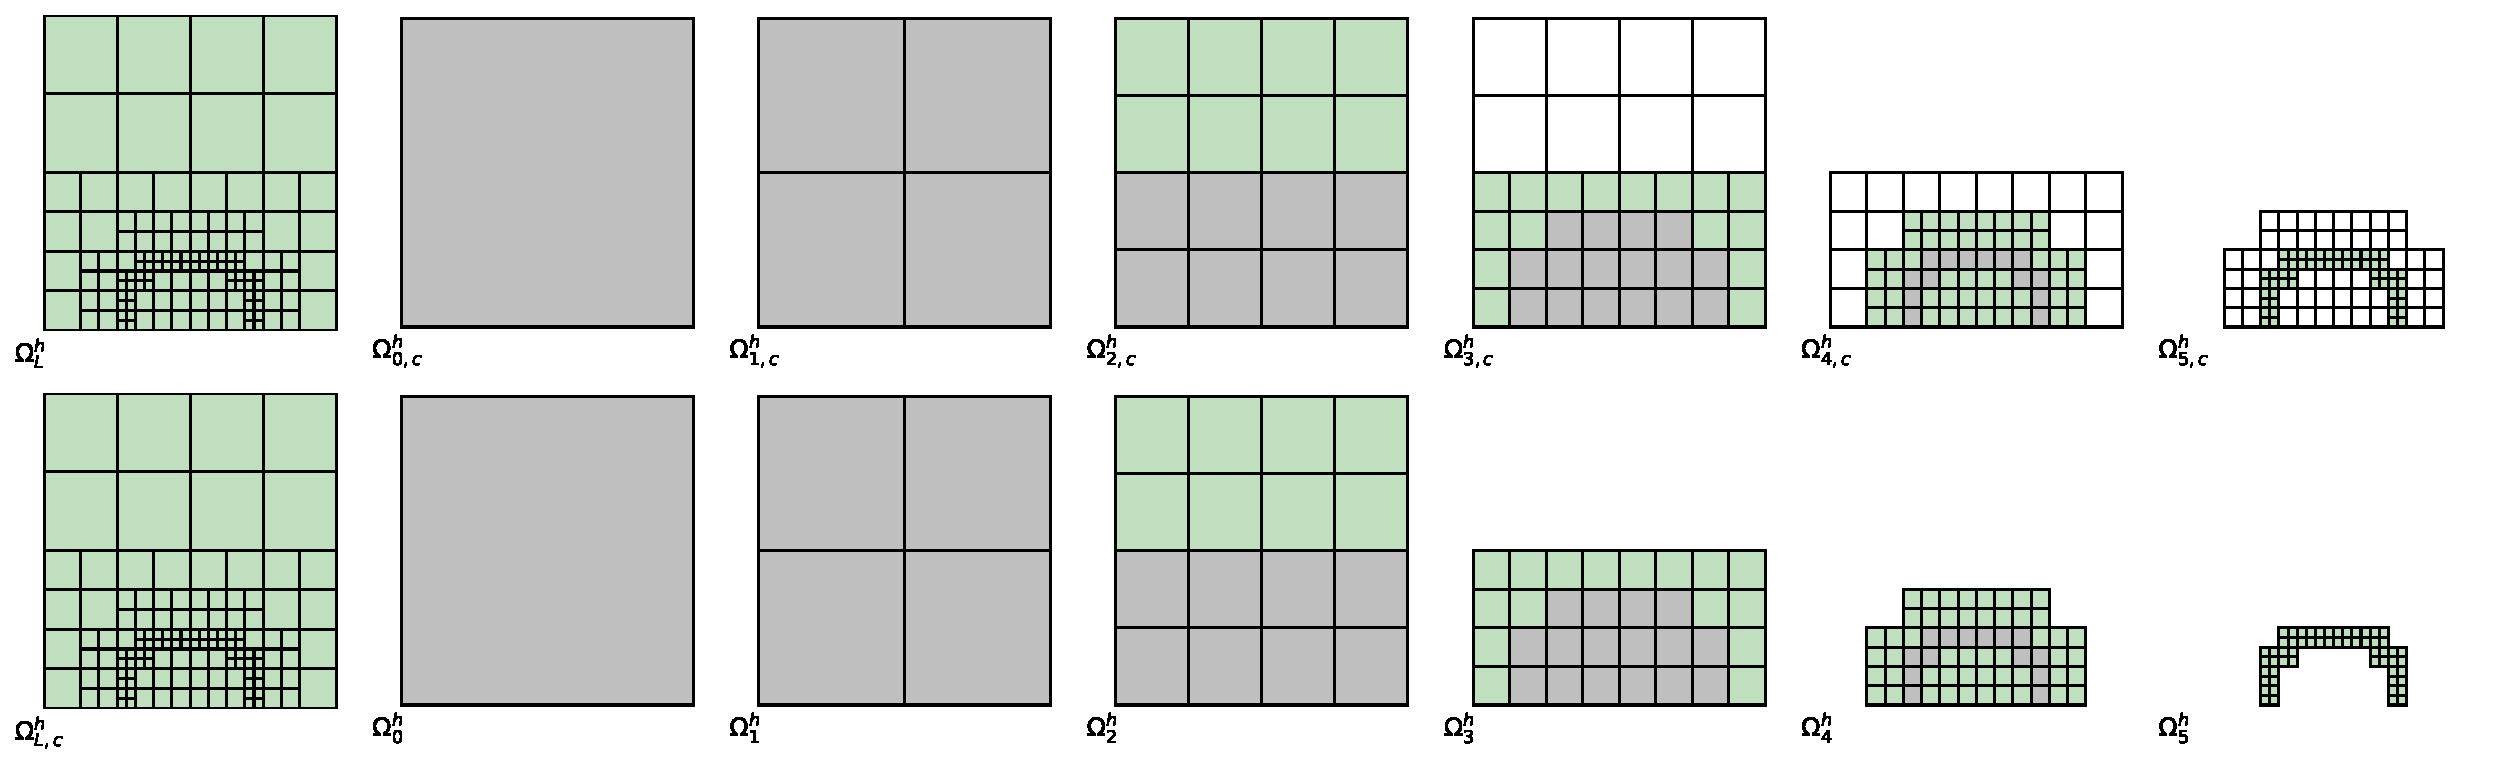
\includegraphics[width=0.95\textwidth]{MG_grid_hierarchy.pdf}
    \caption{Diagram showing the different grids in a multi-grid grid hierarchy for an example Parthenon AMR grid. The squares correspond to blocks in the grid. We do not show grids for negative logical levels since they would appear the same as $\Omega^h_0$ (as coarsening on negative refinement levels occurs by reducing the number of zones per block rather than reducing the number of blocks). Green blocks correspond to leaf nodes, gray blocks correspond to internal nodes in the refinement tree, and uncolored blocks correspond to leaf blocks on the coarser level in a two-level composite grid. Non-course fine boundary neighbor coarse blocks have not been removed from the composite grids, even though they could be. We denote the composite grids by $\Omega^h_{\ell,c}$ instead of $\Omega^h_{\underline{\ell}}$ because of \LaTeX \, issues in matplotlib.}
    \label{fig:grid_hierarchy}
\end{figure}

\subsection{Adaptive Multi-grid} 
Things become somewhat more complex when AMR is included and there are a number of related methods for Adaptive Multi-grid. We use an approach similar to that described in \cite{Trottenburg:2001} Chapter 9 where finer levels do not cover the entire grid. To discuss our algorithm, we need to first formally define the grids that we are working on. Let the domain of our problem (w/o boundary) be $\Omega$ and the boundary of the domain be $\partial \Omega$. We denote a cell-centered grid covering a given domain $\Omega_x$ as $\Omega^h_x$ (and we are generally not careful about explicitly specifying the grid spacing $h$ at different levels). We denote the same grid but including ghost zones as $\bar \Omega^h_x$.  Then we can define some objects: 
\begin{itemize}
    \item {\it Leaf Grid $\Omega^h_L$}: We refer to the pre-existing grid in Parthenon as the leaf grid since it includes all blocks corresponding to leaf nodes in the octree and no blocks corresponding to internal nodes of the refinement octree. Obviously $\Omega_L \cap \Omega = \Omega$. 
    \item {\it Single-level Grid $\Omega^h_\ell$}: A single-level grid for refinement level $\ell$ includes blocks corresponding to all leaf {\it and internal} nodes of the octree at logical level $\ell$. Clearly, for $\ell > \ell_r$ where $\ell_r$ is the level of the Parthenon root grid, we can have $\Omega_\ell \cap \Omega \ne \Omega$. 
    \item {\it Two-level Composite Grid $\Omega^h_{\underline \ell}$}: A two-level composite grid for level $\ell$ that contains all blocks on level $\ell$ and leaf node blocks on level $\ell - 1$ that have neighbors on level $\ell$.\footnote{Currently, the implementation in Parthenon includes all leaf blocks on level $\ell-1$ in $\Omega^h_{\underline \ell}$ but only because including them doesn't impact correctness and it was easier to build the block lists this way. There may be a slight performance boost if only the neighbor blocks are included, but communication on $\Omega^h_{\underline \ell}$ is currently set up so only coarse to fine communication occurs for level $\ell-1$ blocks (and not level $\ell-1$ block to $\ell-1$ block communication).}  To be clear, in our notation in the sub-region $\Omega_{\underline \ell} \cup \Omega_{\ell}$ only cell-centered points from $\Omega^h_{\ell}$ are present while in $\Omega_{\underline \ell} \setminus \Omega_{\ell}$ only cell-centered points from $\Omega^h_{\ell - 1}$ are present.  
\end{itemize}  
An example grid hierarchy is shown in figure \ref{fig:grid_hierarchy}.

We denote a field on level $\ell$ by $\vec{x}_\ell$. Such a field is defined over all of $\Omega^h_\ell$ and has ghost cells in $\bar \Omega^h_\ell \setminus \Omega^h_\ell$. Such a field is only defined once, e.g. the value of $\vec{x}_\ell$ on overlapping regions $\Omega^h_\ell$, $\Omega^h_\underline{\ell}$, $\Omega^h_\underline{\ell - 1}$, and $\Omega^h_L$ is always the same. One consequence of this is that setting the value of a field $\vec{x}_\underline{\ell}$ sets it on $\vec{x}_\ell$ as well. Said in terms of the Parthenon implementation, there is only one block allocated for each node in the tree and multiple blocklists corresponding to different grids can point to the same block. 

\begin{algorithm}

\caption{V-cycle in the Full Approximation Scheme (FAS)\label{alg:FAS}}
\begin{algorithmic}
\Procedure{SMOOTH$_{\ell}$}{$\vec{u}_{\underline \ell}$, $\vec{f}_{\underline \ell}$} \Comment{See note \ref{proc:jacobi}.}
    \State Boundary communication over $\Omega^h_{\underline \ell}$ \Comment{See note \ref{step:composite_boundary_communication}.}
    \State $\vec{t}_\ell \gets A_\ell \vec{u}_\ell \in \Omega^h_\ell$ \Comment{See note \ref{step:smooth_matmult}.}
    \State $\vec{u}_\ell \gets (1 - \omega) D_\ell^{-1} \left(\vec{f}_\ell + D_\ell \vec{u}_\ell - \vec{t}_\ell\right) + \omega \vec{u}_\ell \in \Omega^h_\ell$ \Comment{$\omega = 0$ for undamped Jacobi.}
    \State \Return $\vec{u}_\ell$ 
\EndProcedure
\end{algorithmic}
\begin{algorithmic}
\Procedure{FAS$_{\ell}$}{$\vec{u}_{\underline \ell}$, $\vec{f}_{\underline \ell}$}
    \State $\vec{u}_\ell \gets \text{SMOOTH}_\ell(\vec{u}_{\underline \ell}, \vec{f}_{\underline \ell}) \in \Omega^h_\ell$ 
    \If{$\ell = \ell_{min}$}
      \State \Return $\vec{u}_\ell$
    \EndIf
    \State $\vec{r}_\ell \gets \vec{f}_\ell - A_\ell \vec{u}_\ell \in \Omega^h_\ell$
    \State $\vec{u}_{\underline{\ell-1}} \gets \mathcal{R}^\ell_{\ell - 1} \vec{u}_\ell \in (\Omega^h_{\underline{\ell - 1}} \cap \Omega_\ell)$
    \State $\vec{u}_{\underline{\ell-1}} \gets \vec{u}_{\underline{\ell - 1},0} \in (\Omega^h_{\underline{\ell - 1}} \setminus \Omega_\ell)$ \Comment{See note \ref{step:implicit_u0}.}
    \State $\vec{f}_{\underline{\ell-1}} \gets A_{\ell - 1} \vec{u}_{\ell - 1} + \mathcal{R}^\ell_{\ell - 1} \vec{r}_\ell \in (\Omega^h_{\underline{\ell - 1}} \cap \Omega_\ell)$ \Comment{See note \ref{step:rhs_residual_update}.}
    \State $\vec{f}_{\underline{\ell-1}} \gets \vec{f}_{\underline{\ell - 1},0} \in (\Omega^h_{\underline{\ell - 1}} \setminus \Omega_\ell)$ \Comment{See note \ref{step:implicit_u0}.}
    \State $\vec{v}_{\ell - 1} \gets \textrm{FAS}_{\ell - 1}(\vec{u}_{\underline{\ell-1}}, \vec{f}_{\underline{\ell - 1}}) \in \Omega^h_{\ell - 1}$
    \State $\vec{e}_{\ell - 1} \gets \vec{v}_{\ell - 1} - \vec{u}_{\ell - 1} \in \Omega^h_{\ell - 1}$ 
    \State $\vec{u}_{\underline \ell} \gets \vec{u}_{\underline \ell} + \mathcal{P}^{\ell-1}_{\underline \ell} \vec{e}_{\ell - 1} \in \Omega^h_\ell $
    \State $\vec{u}_\ell \gets \text{SMOOTH}_\ell(\vec{u}_\ell, \vec{f}_\ell) \in \Omega^h_\ell$
    \State \Return $\vec{u}_\ell$
\EndProcedure 
\end{algorithmic} 
\end{algorithm}

The FAS based adaptive MG algorithm that is implemented in Parthenon is described in algorithm \ref{alg:FAS}. I {\it think} this is essentially similar to the Fast Adaptive Composite (FAC) algorithm of McCormick, maybe even exactly the same, but it is challenging to translate some of the literature to cell-centered schemes and the block-based AMR language. Some specific details of the algorithm are:
\begin{enumerate}
    \item\label{proc:jacobi} We write the smoother as a Jacobi iteration for simplicity of presentation, but in practice we usually use multiple scheduled Jacobi iterations where $\omega$ varies in a prescribed way with each iteration \cite{Yang:2017}. 
    \item\label{step:composite_boundary_communication} We fill all boundaries of blocks at level $\ell$ contained in $\Omega^h_{\underline \ell}$. Prolongating values from blocks on level $\ell - 1$ to the ghost zones of blocks on level $\ell$ is key to achieving good convergence\footnote{Initially, we just tried setting the ghost zones of fine blocks at coarse-fine boundaries on composite grids to a constant value given by a initial communication over the entire leaf grid. Then, when prolongating the error from a coarser grid $\Omega^h_{\ell-1}$ to a finer grid $\Omega^h_\ell$, we reset the coarse-fine boundaries of the fine grid based on prolongating from leaf and internal blocks on $\Omega^h_{\ell-1}$. In both cases the coarse-fine boundaries were not updated during the smoothing operations. This resulted in an MG algorithm that converged similarly to the algorithm we settled on when doing raw V-cycles, but when used as a single v-cycle preconditioner with BiCGStab this algorithm failed miserably (i.e. it often did not converge at all on AMR problems that both MG alone and BiCGStab alone would converge on). It appears that the effective lag in updating the coarse-fine boundaries resulted in large residuals on the fine grid next to the coarse-fine boundaries.} with the multilevel algorithm. Since the $\ell$ boundary values are interpolated, they depend on both non-ghost cells in the neighboring $\ell - 1$ block {\it and} non-ghost cells in the block on $\ell$ itself (think of the prolongation stencil).  
    \item\label{step:smooth_matmult} The operator $A_\ell$ only returns an answer in the grid $\Omega^h_\ell$ but it will almost always reach into ghost values in $\bar \Omega^h_\ell \setminus \Omega^h_\ell$. Because of interpolation into these coarse-fine boundaries, this introduces further dependence on values in $\Omega^h_\ell$ near the boundary, as well as dependence on $\Omega^h_{\ell-1} \setminus \Omega_\ell$. As a result the true diagonal of the matrix may get an extra contribution from where the single level representation of $A$ (that is $A_\ell$) reaches into the boundaries. We have found that it is likely safe to neglect this extra contribution to $D$ and use the value of $D$ that would be found for a uniform grid.
    \item\label{step:implicit_u0} Steps updating coarse zones on two-level composite grids are not explicitly included in the task list, since it is already performed for all levels by initializing $\vec{u}_L \gets \vec{u}_{0,L}$ (and similarly for $\vec{f}_L$ before starting the FAS). 
    \item\label{step:rhs_residual_update} We can cast this in terms of $\tau$ corrections $A_{\ell - 1} \vec{u}_{\ell - 1} + \mathcal{R}^\ell_{\ell - 1} \vec{r}_\ell = \mathcal{R}^\ell_{\ell - 1} \vec{f}_\ell + \tau^\ell_{\ell - 1}$ where the correction to the restricted RHS is $\tau^\ell_{\ell - 1} = A_{\ell - 1} \mathcal{R}^\ell_{\ell - 1}  \vec{u}_\ell -  \mathcal{R}^\ell_{\ell - 1} A_\ell \vec{u}_\ell$. We can then consider the $\tau$ correction of the composite grid $\tau^{\underline{\ell}}_{\ell - 1} = A_{\ell - 1} \mathcal{R}^{\underline{\ell}}_{\ell - 1}  \vec{u}_{\underline{\ell}} -  \mathcal{R}^{\underline{\ell}}_{\ell - 1} A_{\underline{\ell}} \vec{u}_{\underline{\ell}}$, where $\mathcal{R}^{\underline{\ell}}_{\ell - 1}$ is just the identity outside of $\Omega^h_\ell$ and rows of $A_{\underline{\ell}}$ outside $\Omega^h_\ell$ that do not reach into the fine region are the same as $A_{\ell-1}$. In fact for Poisson like problems, if we don't include flux correction, $A_{\underline{\ell}} = A_{\ell - 1} \in \Omega^h_{\ell - 1} \setminus \Omega_{\ell}$ (for rows). That suggests that if we do want to include flux correction in MG, it may be best done through a $\tau$ correction. Obviously, flux correction is not present in the single level operator $A_\ell$ but there would be a contribution from flux correction to $A_{\underline{\ell}}$ on the coarse side of the coarse-fine boundary inside the two-level grid. This would result in a non-zero value for $\tau^{\underline{\ell}}_{\ell - 1}$ at the internal boundary of $\Omega^h_{\ell-1} \setminus \Omega_{\ell}$ and a slight correction to the input RHS on coarse-fine boundary leaf blocks on level $\ell - 1$. I also think that after every v-cycle, $\vec{f}_L$ would have to be reset to $\vec{f}_{0,L}$. An original reference for this is \cite{Bai:1987}. That being said, it appears that using un-flux corrected MG as a preconditioner for flux-corrected BiCGStab seems to work just fine so this addition seems unnecessary for the time being.
\end{enumerate}

Some notes about the specific implementation in Parthenon: 
\begin{enumerate} 
\item Restriction is performed using the standard Parthenon \texttt{RestrictAverage} method, which is clearly linear. The default shared prolongation operator is not linear, since it is slope limited, so we use the prolongation operator \texttt{ProlongateSharedLinear} that performs bi/trilinear interpolation from a coarse grid to a fine grid. Fields involved in MG need to have this (or another) linear prolongation operator registered for the adaptive MG procedure to be linear. The default internal prolongation operator, \texttt{ProlongateInternalAverage}, is linear so no change is required there (and it also doesn't play a role for cell-centered fields). The linear prolongation operator should work with fields of any topological type.
\item Physical boundary conditions need to be carefully constructed so that they are implemented consistently on $\partial \Omega$ at all levels of the grid. Setting the ghosts to a constant value will not work since the position of the ghost points on the physical boundaries changes as the refinement level is changed. For Dirichlet boundary conditions, we find the choosing ghost points so that the value of the field linearly interpolated to the face between the ghost and the first active zone satisfies the Dirichlet condition. For nodal fields and face fields, it may be better to impose boundary conditions on the first layer of internal zones that sit on the boundary face\footnote{There is probably room for some careful thinking about how we want to impose boundary conditions on non-cell centered fields in general.}.
\item Below the Parthenon root grid, we coarsen as many times as possible de-refining by a factor of two. The number of possible de-refinements from the root grid, $\alpha$, is given by the minimum $\alpha_d$ amongst all directions $d$ where $\alpha_d$ for each direction is the the maximum value of $\alpha_d$ for which $(n_{r,d} \times n_{z,d}) \bmod 2^{\alpha_d} = 0$. Here $n_{r,d}$ is the number of blocks in the $d$ direction at the level of the root grid and $n_{z,d}$ is the number of zones in the $d$ direction in blocks at or finer than the root grid level. Above the root grid, this can result in blocks that are not all the same shape, even across a single refinement level\footnote{Dealing with this possibility generically requires the use of hierarchical parallelism within Parthenon kernels that loop over blocks, since the spatial index range can change amongst blocks in a single \texttt{MeshData} object. Obviously this is not required if grid sizes are chosen judiciously so blocks on a single level always have the same shape (even if the block size varies between refinement levels)}. If $\alpha$ is larger than the level of the root grid, this leads us to define ``negative'' logical levels within our grid hierarchy. At logical level zero, a single block covers $\Omega$. For negative levels, a single block still covers $\Omega$ but this block will have a factor of two coarser zones in every direction than the block on the next higher level.
\end{enumerate} 

\subsection{Results}

\begin{figure}[!htb]
    \centering
    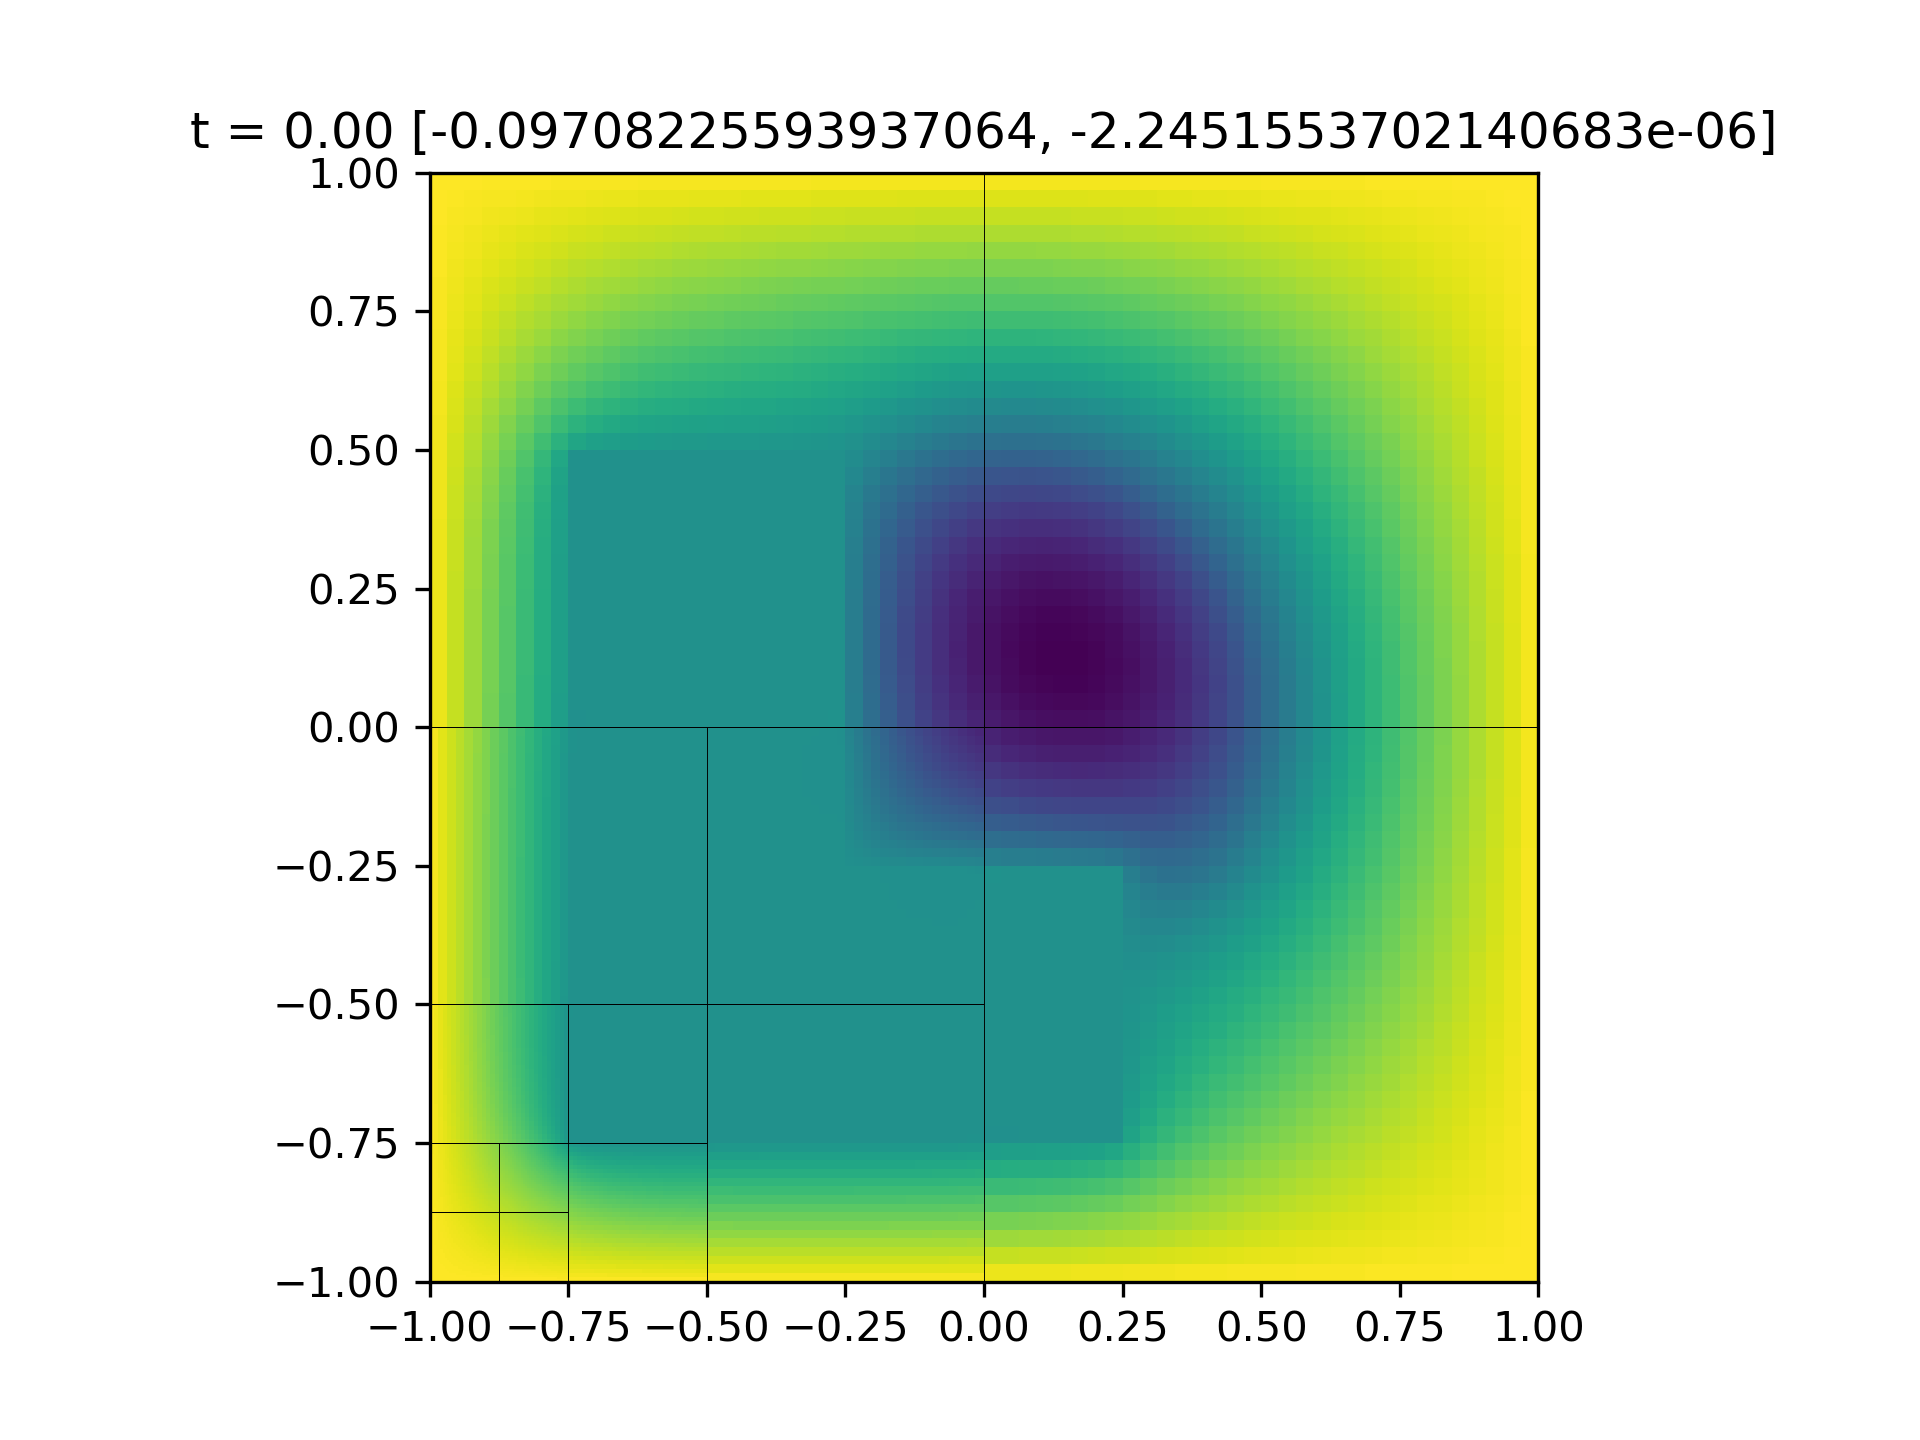
\includegraphics[width=0.49\textwidth]{x.png}
    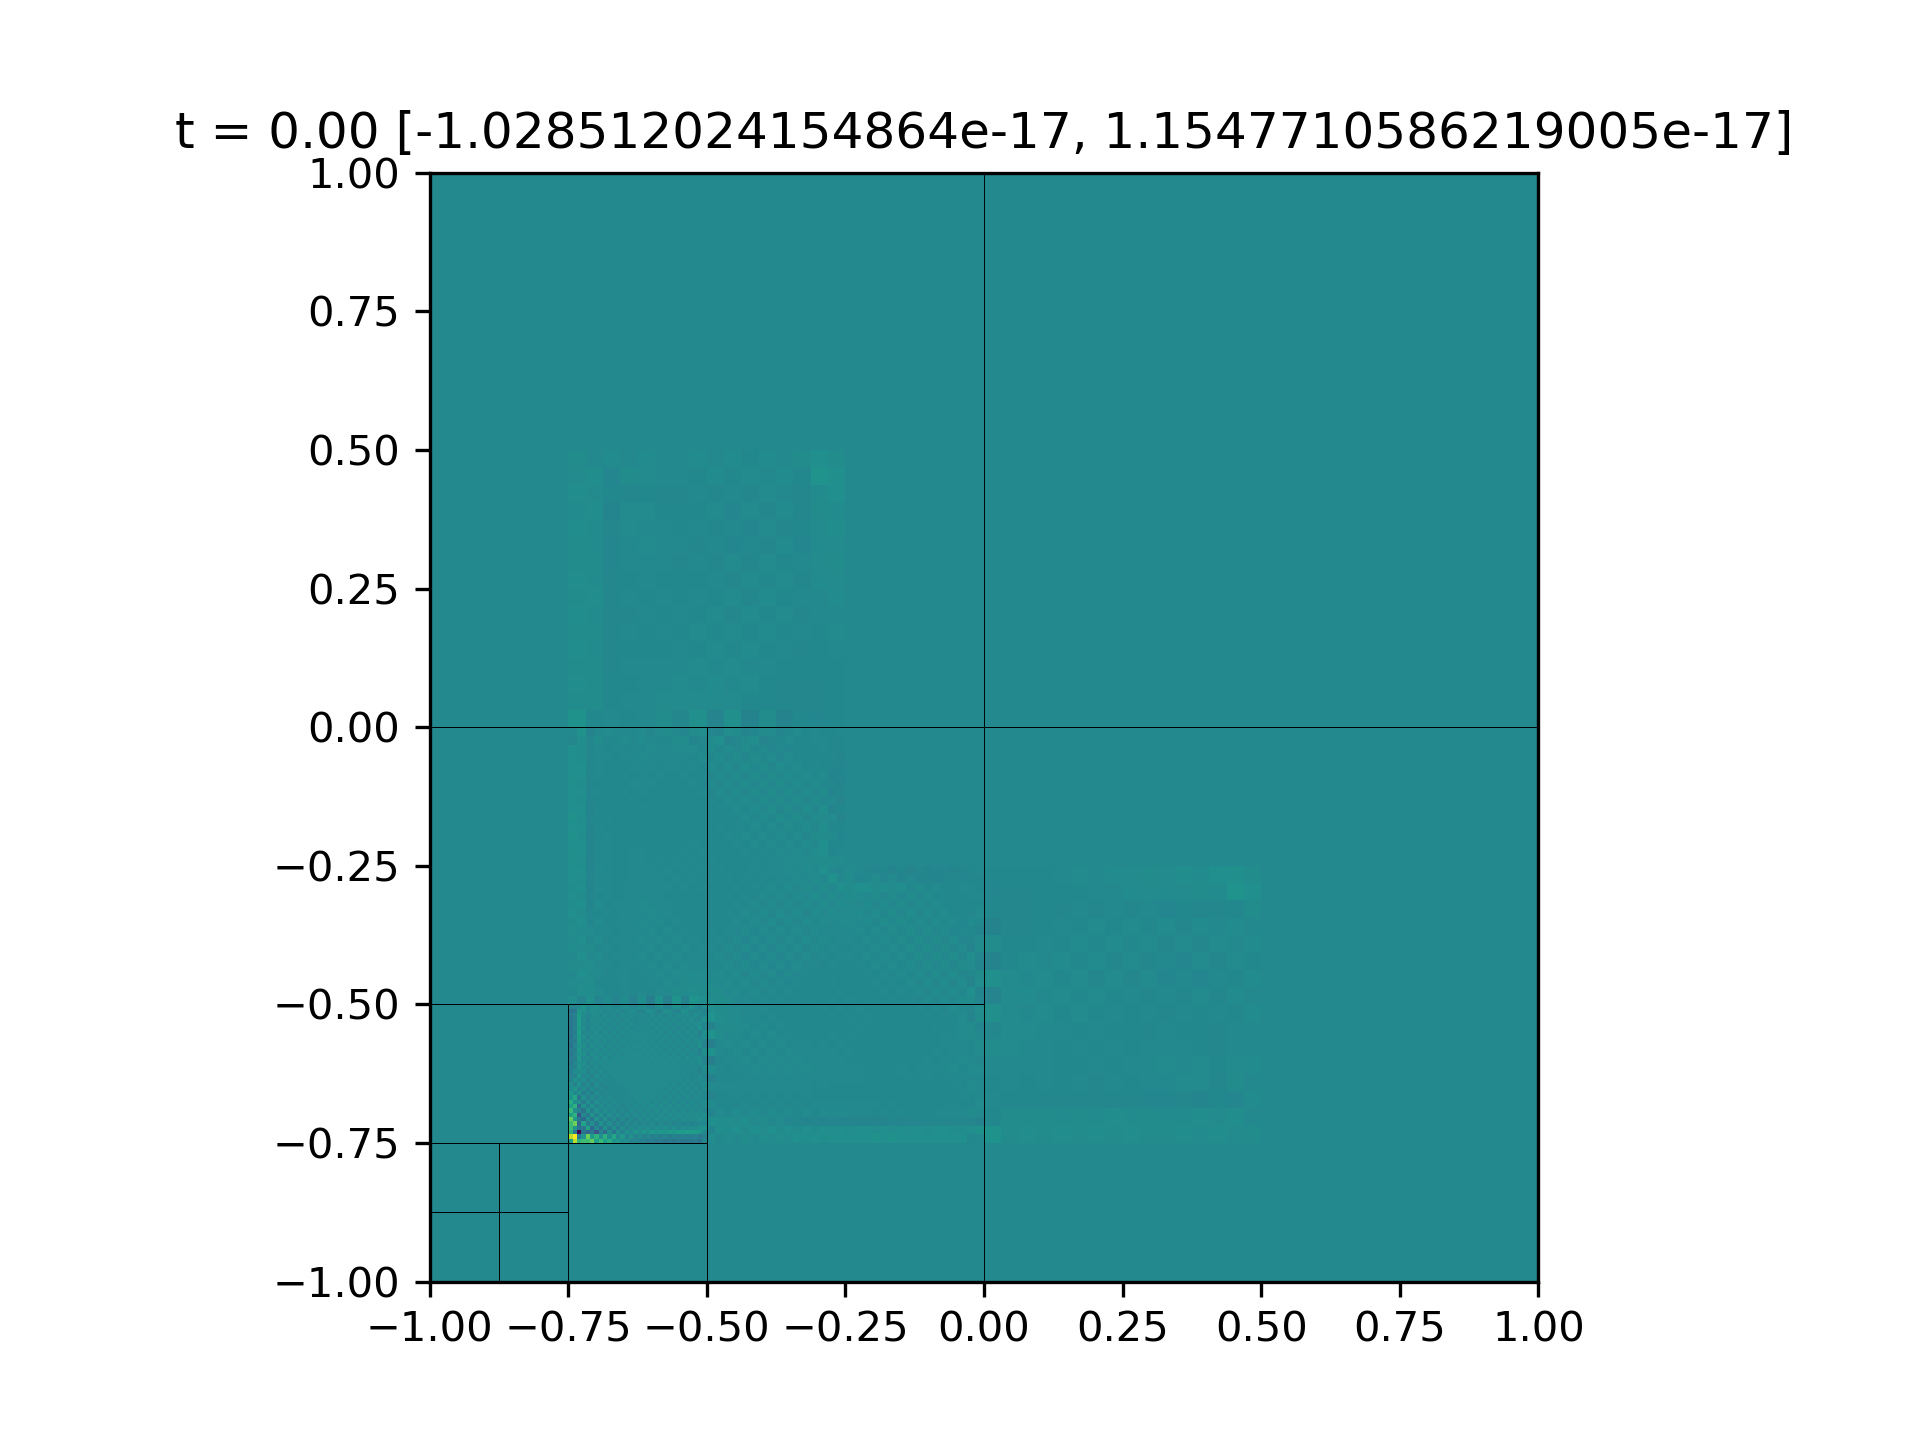
\includegraphics[width=0.49\textwidth]{r.png}
    \caption{Example solution and residuals found for a discretized version of the equation $\nabla \cdot D \nabla u = f$, where $D=1000$ in the L-shaped region and $D=1$ elsewhere. The source function $f$ is one inside a radius of 0.5 and zero elsewhere and $u=0 \in \partial \Omega$.}
    \label{fig:solution}
\end{figure}

\begin{figure}[!htb]
    \centering
    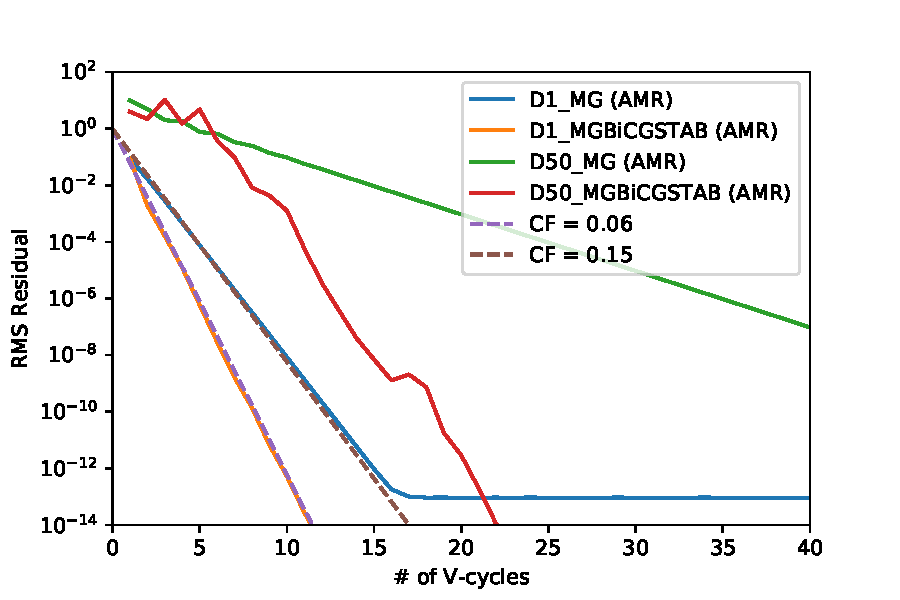
\includegraphics[width=0.7\textwidth]{convergence.pdf}
    \caption{Convergence properties of the MG implementation in Parthenon for the problems similar to that shown in figure \ref{fig:solution}. D1 corresponds to $D=1$ throughout the whole grid, while D50 corresponds to $D=50$ within the L-shaped region.}
    \label{fig:convergence}
\end{figure}

\bibliographystyle{plainurl}
\bibliography{parthenon}

\end{document}
